% *//   MODELE DE DOCUMENT LaTeX //* 
% -----------------------------------
% Inclut sections, sous-sections et sous-sous-sections.
% Examples d'intégration de figures, de tableaux et d'algorithme.
% -----------------------------------
% Gestion automatique de la mise en forme biblio grâce à BibTeX.
% Il suffit de copier le code BibTeX de la publication dans le fichier 'biblio.bib'.
% Sur GScholar : cliquer sur Citer puis BibTeX.
% Citer ensuite le papier comme dans l'example de l'introduction. 
% La bibliographie sera automatiquement mise en forme à la fin du document aux normes APA. 
% -----------------------------------
\documentclass[11pt]{article}
\usepackage[utf8]{inputenc}
\usepackage{graphicx,setspace,csquotes}
\usepackage{amsmath}
\usepackage[T1]{fontenc}
% Police Helvetica pour tout le texte
\usepackage{helvet}
\renewcommand{\familydefault}{\sfdefault}
\usepackage[skip=10pt, indent=25pt]{parskip}
\usepackage[english,french]{babel}
\usepackage[autolanguage]{numprint}
\usepackage[backend=biber,style=apa,sorting=nyt]{biblatex}
\DefineBibliographyExtras{french}{%
  \restorecommand\mkbibnamefamily
}
\usepackage[font=small,labelfont=bf]{caption}
\usepackage[left=2cm, right=2cm, top=2.5cm, bottom=2.5cm]{geometry}
\usepackage{booktabs}
\usepackage[french]{algorithm2e}
\usepackage{float}
\usepackage{hyperref}
\def\frenchtablename{Tableau}
\usepackage{caption}
\usepackage{subcaption}
\usepackage[dvipsnames]{xcolor}
\usepackage{tabularx}
%\usepackage{enumitem}

\addbibresource{biblio.bib}

% Configuration des liens
\definecolor{personalizedColor}{RGB}{0, 163, 166}
\hypersetup{
    colorlinks=true,
    linkcolor=black,
    filecolor=black,      
    urlcolor=personalizedColor,
    citecolor=personalizedColor,
    pdftitle={Prévision de la consommation électrique en France},
    pdfpagemode=FullScreen,
    }
\urlstyle{same}
% Configuration des algorithmes
\RestyleAlgo{ruled}
\SetKw{KwBy}{by}
% Configuration des légendes
\captionsetup{width=13.5cm}

% Eviter les pages presque vides reservees aux figures.
\renewcommand{\topfraction}{0.9}
\renewcommand{\bottomfraction}{0.9}
\renewcommand{\textfraction}{0.08}
\renewcommand{\floatpagefraction}{0.8}
\begin{document}

\hypersetup{pageanchor=false}
\begin{titlepage}
    \begin{center}
        \vspace*{0.5cm}
        \LARGE
        \textbf{Watt's demain: Algorithme de prédiction des données de consommation électrique française}\\
            
        \vspace{1cm}
        \Large
        \textbf{Melissa Aliouche, Nada Haddad, Lola Cusin}\\
        M2 Machine Learning for artifical Intelligence (MALIA)\\
        \vspace{0.5cm}
        \large
        \textbf{11/11/2026}\\
            
        \vfill

% Image absente du template : \includegraphics[width=0.20\textwidth]{logos/logo1.png}
        
        %\includegraphics[width=0.25\textwidth]{logos/logo2.png}
        
% Image absente du template : \includegraphics[width=0.15\textwidth]{logos/logo2.png}
% Image absente du template : \includegraphics[width=0.15\textwidth]{logos/logo2.png}
% Image absente du template : \includegraphics[width=0.15\textwidth]{logos/logo2.png}
        
        \textbf{Cours: } Temporal Data Analysis\\        
        \textbf{Enseignant: } Jairo Cugliari
        
    \end{center}
\end{titlepage}

\setstretch{1.2}

\pagenumbering{gobble}

\tableofcontents
\newpage

\hypersetup{pageanchor=true}
\section{Introduction}
\pagenumbering{arabic}

\noindent

Afin d'assurer le bon fonctionnement du réseau électrique, il est nécessaire d'avoir un équilibre entre la production et la consommation d'électricité. La consommation d'électricité est influencée par de nombreux facteurs, tels que la météo, les habitudes de consommation des ménages et des entreprises, et les événements spéciaux. La prévision de la consommation d'électricité est donc un enjeu crucial pour les gestionnaires de réseau: elle permet d'anticiper les besoins, de planifier la production et donc de de garantir la stabilité du système électrique. 

Afin de suivre la consommation électrique en temps réel, le Réseau de Transport d’Électricité RTE collecte les données de consommation à l'aide de télémesures transmises directement depuis ses installations \parencite{rte_eco2mix_2026}. Certains de ses sites ne sont pas équipé pour la télémesures, les données sont donc complétées par des estimations, remplacées par la suite par des données de comptage plus complètes. RTE propose également des prévisions de consommation à court terme, qui sont utilisées pour planifier la production et la distribution d'électricité. Ces prévisions sont basées sur des modèles statistiques et des algorithmes de machine learning, qui prennent en compte les données historiques de consommation, les conditions météorologiques et d'autres facteurs pertinents.

L'objectif de ce rapport est de proposer un algorithme de prédiction de la consommation électrique française à court terme, en utilisant les données de consommation collectées par RTE. Nous allons explorer différentes approches de modélisation, en utilisant des techniques d'analyse de séries temporelles et de machine learning, afin d'obtenir des prévisions précises et fiables. Nous allons également évaluer les performances de notre algorithme en le comparant à des benchmarks, des modèles statistiques et ainsi qu'à d'autres modèles de machine learning, et en analysant les erreurs de prévision pour identifier les points faibles et les opportunités d'amélioration. Nos prédictions s'appuieront sur les données historiques compilées par RTE, ainsi que sur les données météorologiques du réseau SYNOP \parencite{meteo_france_synop_2026}, et le calendrier des jours fériés et vacances scolaires en France.


\section{Méthodes}
\noindent

\subsection{Récupération et préparations des données}
\noindent

\subsubsection{Sources et périmètre}


\begin{table}[H]
    \centering
    \fontsize{10}{12}\selectfont
    \renewcommand{\arraystretch}{1.3}
    \caption{Source des données utilisées pour l'analyse et la modélisation.}
    \begin{tabularx}{\linewidth}{p{2.5cm} X X X X X}
        \toprule
        Données & Source & Période \newline disponible & Granularité initiale & Variables \newline retenues & Unités \\
        \midrule
        Consommation \newline électrique & \cite{rte_eco2mix_2026} & Depuis 2012 & 30 minutes & Consommation & MWh \\
        Météo & \cite{meteo_france_synop_2026} & Depuis 1996 & 3 heures & Température, précipitations & ° K, mm \\
        Calendrier & N/A & N/A & 1 jour & Date, jours \newline fériés et \newline vacances & N/A \\
        \bottomrule
    \end{tabularx}
    
    \label{tab:scenarios}
\end{table}

\subsubsection{Construction du tableau horaire}

- Consommation : nettoyage, agrégation des demi-heures et convention retenue pour dater la moyenne. \newline
- Météo : stations métropolitaines retenues, seuil de couverture de la température et des précipitations, moyenne spatiale à poids égaux, conversion des unités et reconstruction horaire. \newline
- Préciser que l'écart-type météo mesure la dispersion entre stations, pas l'incertitude de la moyenne nationale.\newline
- Calendrier : jour, heure, week-end, jours fériés et vacances par zone ; justification des variables retenues.\newline
- Jointure temporelle, vérification du fuseau RTE, traitement des doublons, valeurs manquantes et observations atypiques.\newline
- Changements d'heure : expliquer la convention permettant de traiter la demande de 24 cibles malgré les journées françaises de 23 ou 25 heures ; documenter toute exclusion.

\subsubsection{Analyse exploratoire}

Explorer les données d'apprentissage pour orienter les modèles sans utiliser le test final pour choisir les variables.

- Cycles journalier et hebdomadaire, saisonnalité annuelle. \newline
- Relation température–consommation et effets calendaires.\newline
- Tendances, ruptures de régime et observations atypiques, sans suppression automatique des événements réels.

Figures proposées : profils horaires et saisonniers ; relation température–consommation ou de série longue montrant les ruptures. 


\subsection{Benchmarks et modèles}
\noindent

\begin{algorithm}[h]
    \caption{Un superbe algorithme}\label{alg:justanalgorithm}
    \textit{Entrées}
    \begin{itemize}
        
        \item[$\bullet$] $Variable = $ description de la variable
        \item[$\bullet$] $Variable = $ description de la variable
        \item[$\bullet$] $Variable = $ description de la variable
        \item[$\bullet$] $Variable = $ description de la variable
    \end{itemize}
    \textit{Initialisations}
    \begin{itemize}
        \item[$\bullet$] $Variable = valeur$
        \item[$\bullet$] Effectuer une action
    \end{itemize}
    \textit{Calculs}\\
        \For{$variable \gets 0$ \KwTo $Variable$ \KwBy $1$}{
            \ForEach{$truc \in machin$}{
                Faire à $truc$ quelque chose prenant en compte $Variable$ \\
                Mise à jour de $machin$
            }
        $Variable = Variable \times Variable$
        }
    \textit{Sorties}
    \begin{itemize}
        \item[$\bullet$] Ce que l'on sort de l'algorithme
    \end{itemize}
\end{algorithm}

\subsection{Validation chronologique et métriques}
\noindent

\subsubsection{Sous-sous-section}
\noindent


% !TeX root = main.tex
\section{Résultats}\label{sec:resultats}

\subsection{Exploration et couverture des données}
Les critères de couverture retiennent 37 stations SYNOP. Sur la grille géographique utilisée, 45,1\,\% de la surface métropolitaine est à moins de 50~km d'une station et 97,3\,\% à moins de 100~km (distance médiane : 53,0~km). La carte montre une proximité géographique, sans démontrer une représentativité climatique ou démographique.

\begin{figure}[htbp]
  \centering
  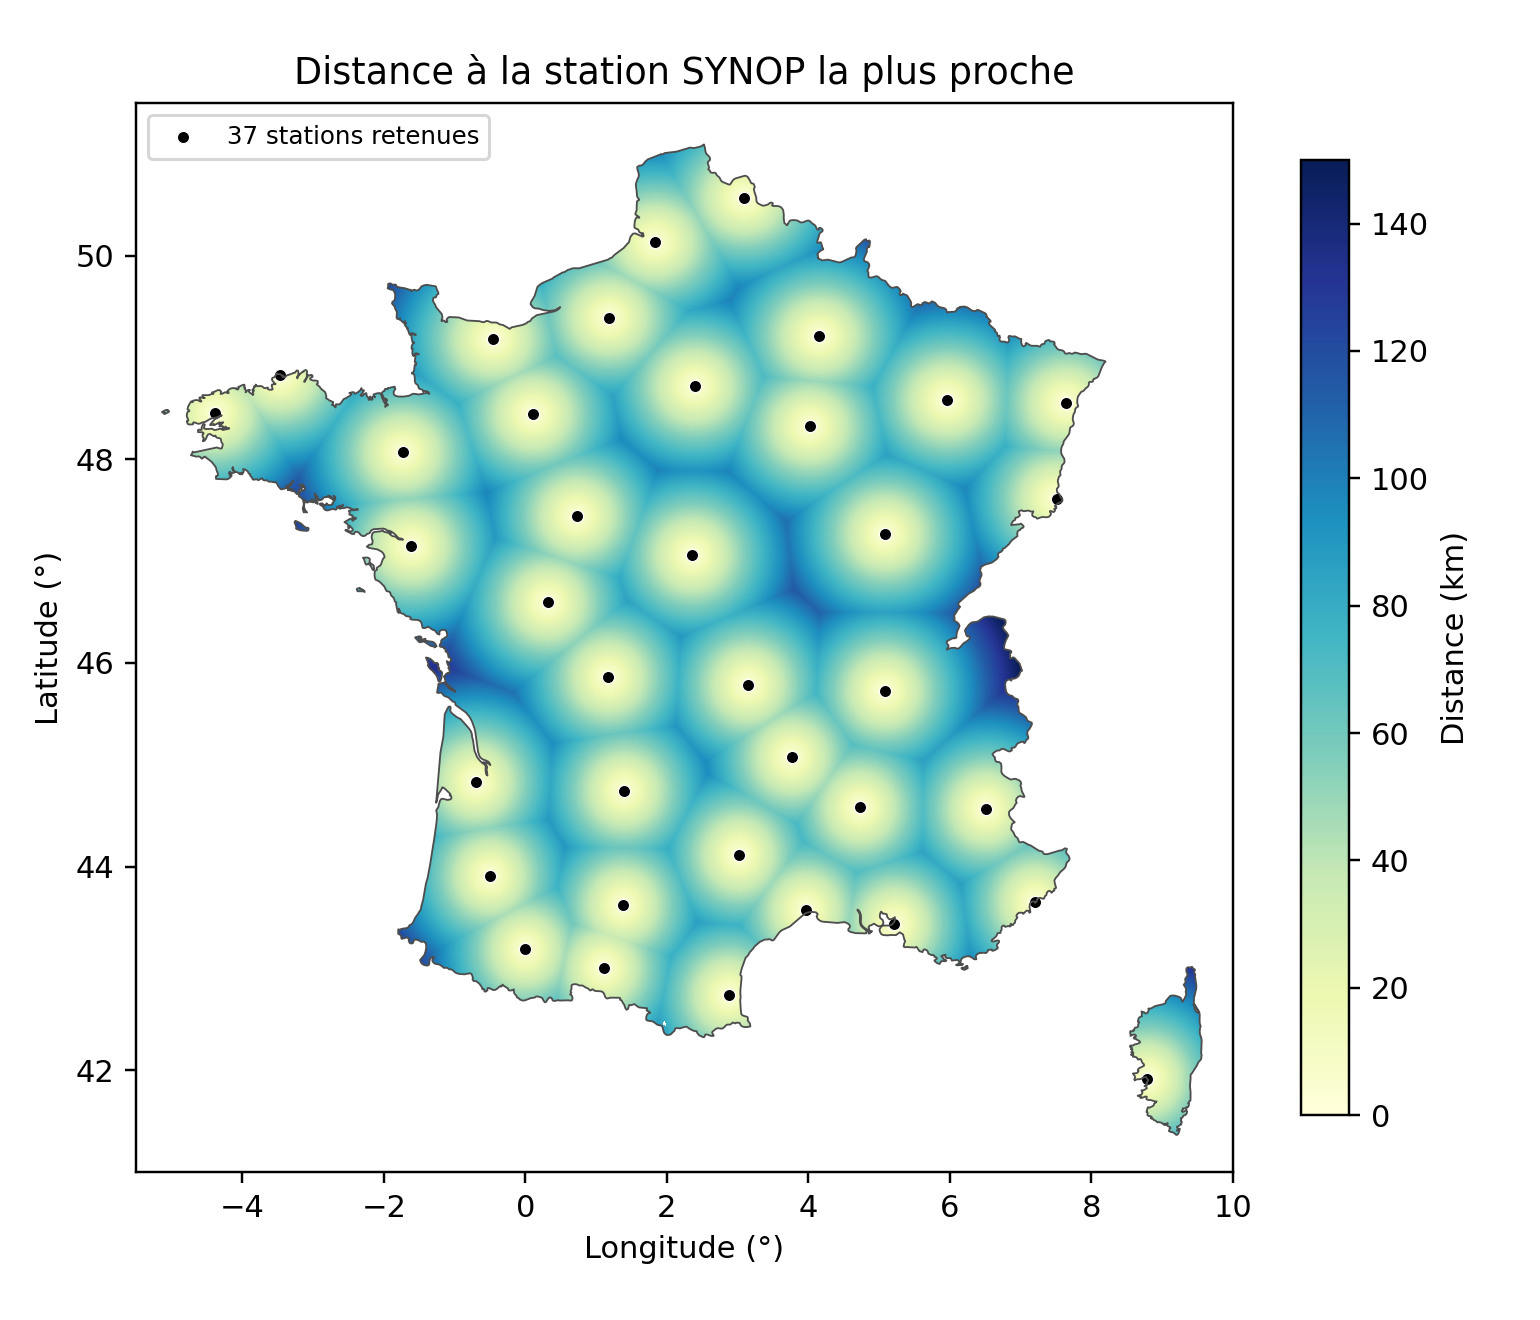
\includegraphics[width=.48\linewidth]{../results/analyse_2024/couverture_geographique/couverture_geographique.png}
  \caption{Distance à la station SYNOP retenue la plus proche.}\label{fig:stations}
\end{figure}

Les profils moyens sur l'apprentissage 2012--2023 mettent en évidence les cycles journalier et hebdomadaire (figure~\ref{fig:profils}). La consommation moyenne par mois est plus élevée en hiver qu'en été ; les mois froids coïncident aussi avec les consommations les plus fortes. Le graphique comparant les vacances scolaires montre des niveaux médians différents, sans isoler leur effet de celui de la saison ou du jour de la semaine. Ces constats descriptifs motivent les variables calendaires et météorologiques. La différence à 168~h atténue certains motifs hebdomadaires, sans éliminer nécessairement la tendance ni rendre la série stationnaire.
\begin{figure}[htbp]
  \centering
  \begin{subfigure}{.46\linewidth}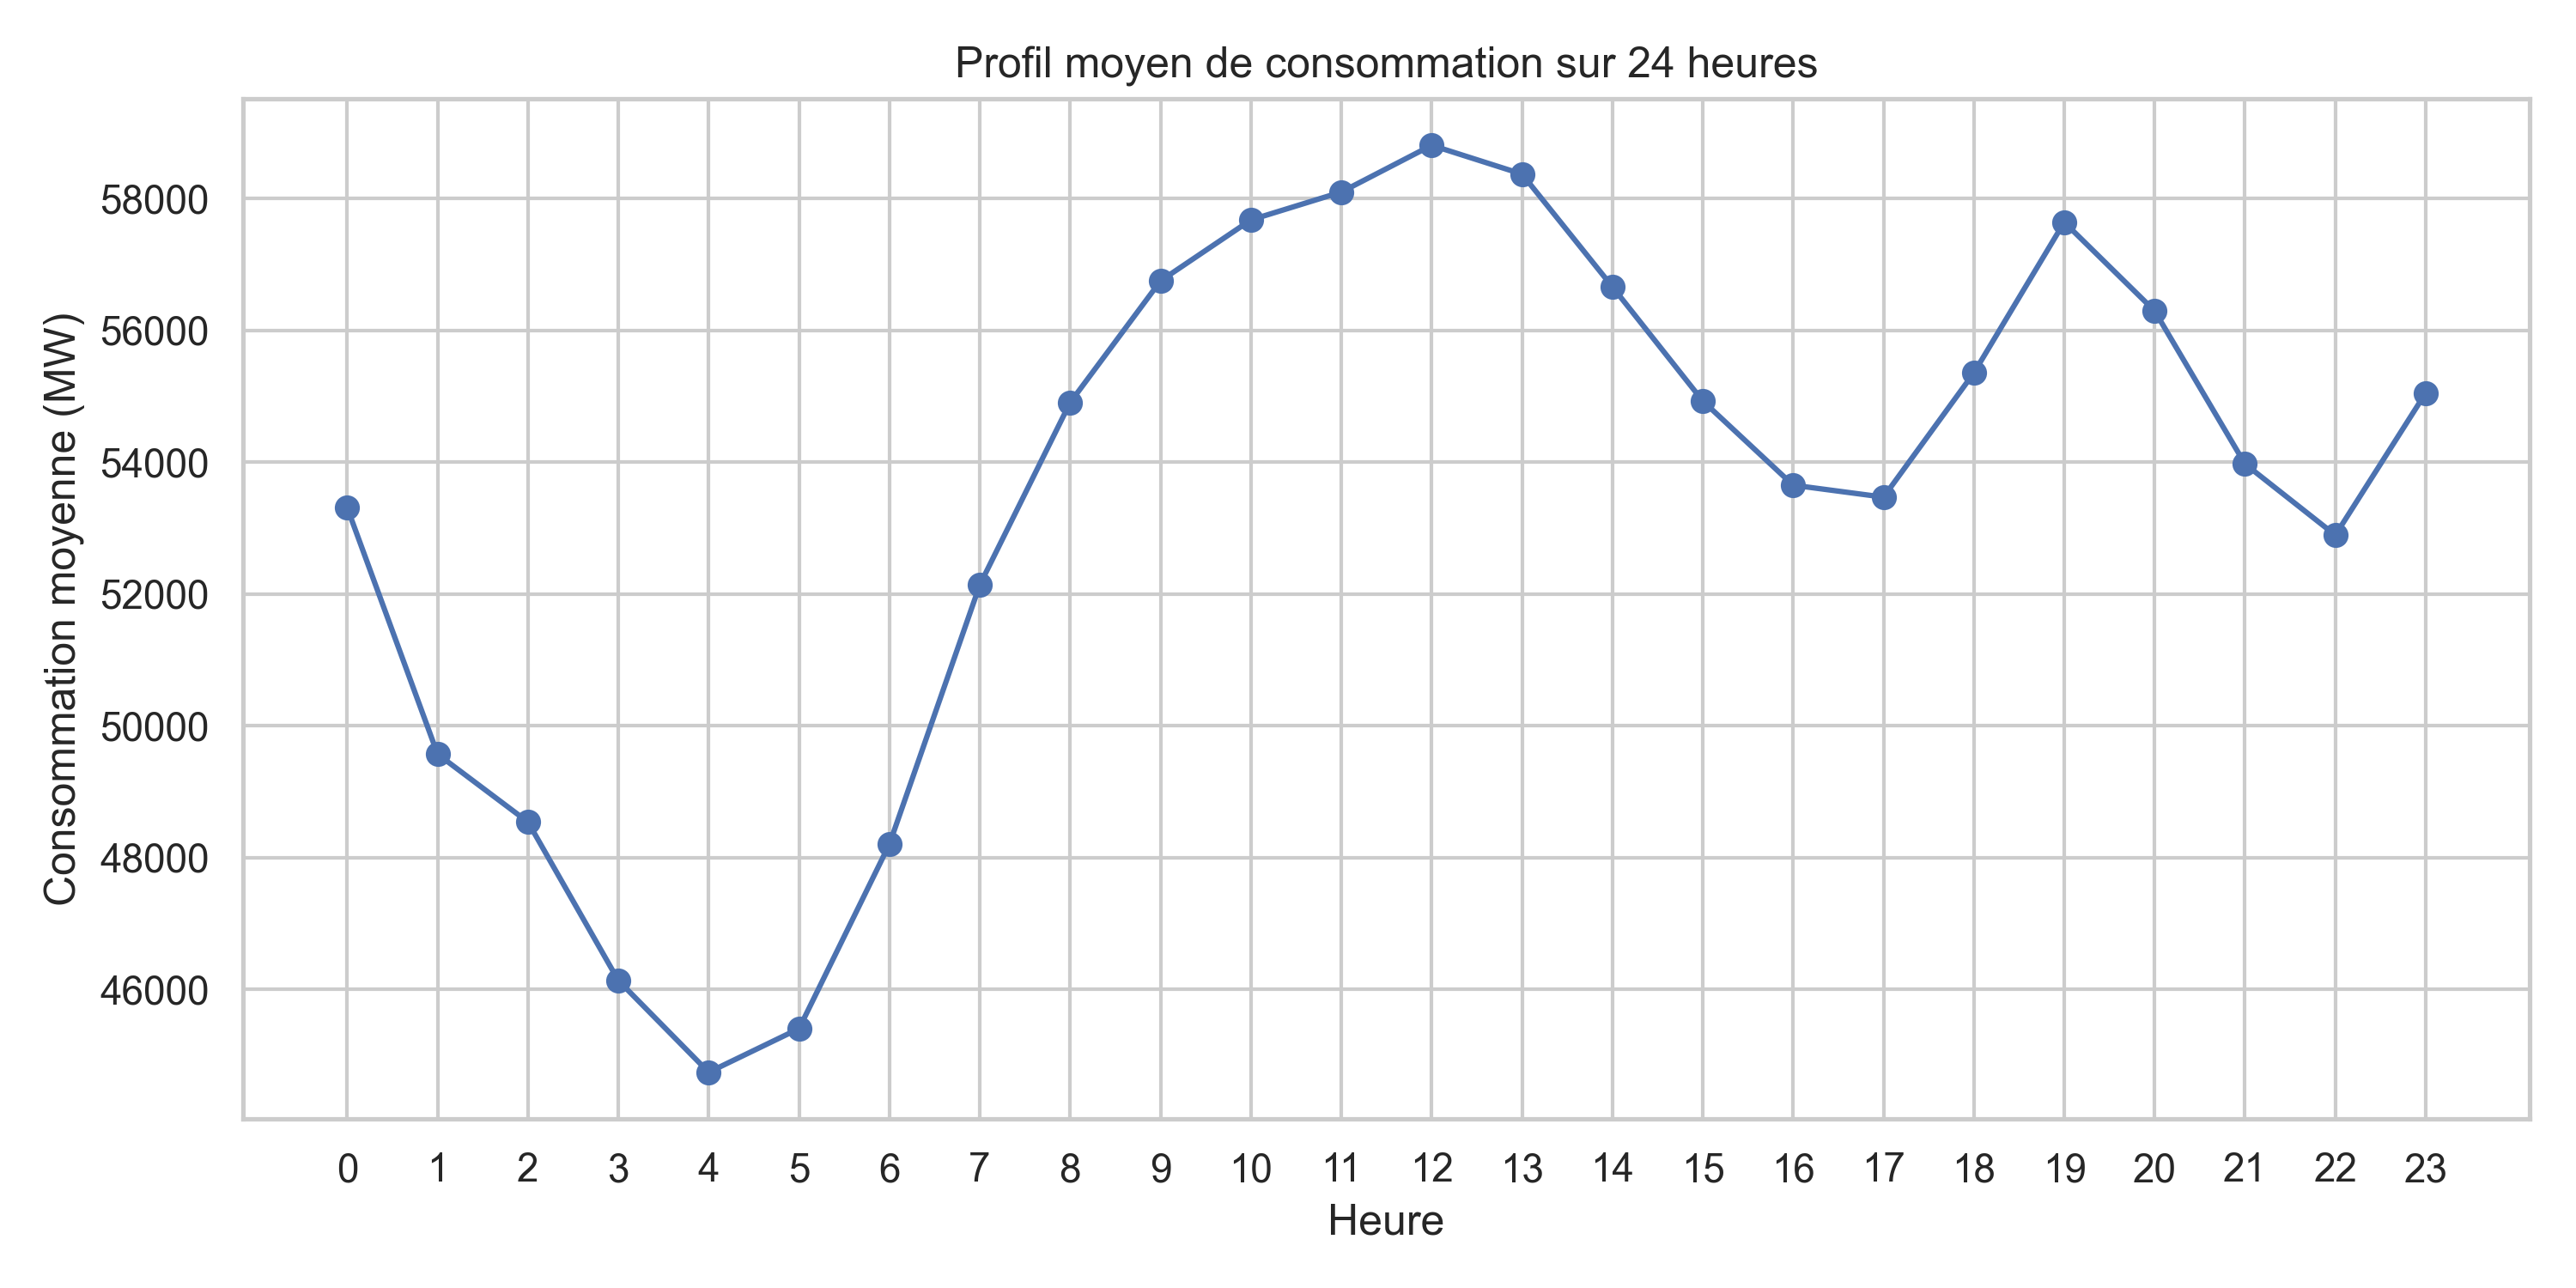
\includegraphics[width=\linewidth]{../results/analyse_2024/exploration/cycle_journalier.png}\caption{Cycle journalier.}\end{subfigure}\hfill
  \begin{subfigure}{.46\linewidth}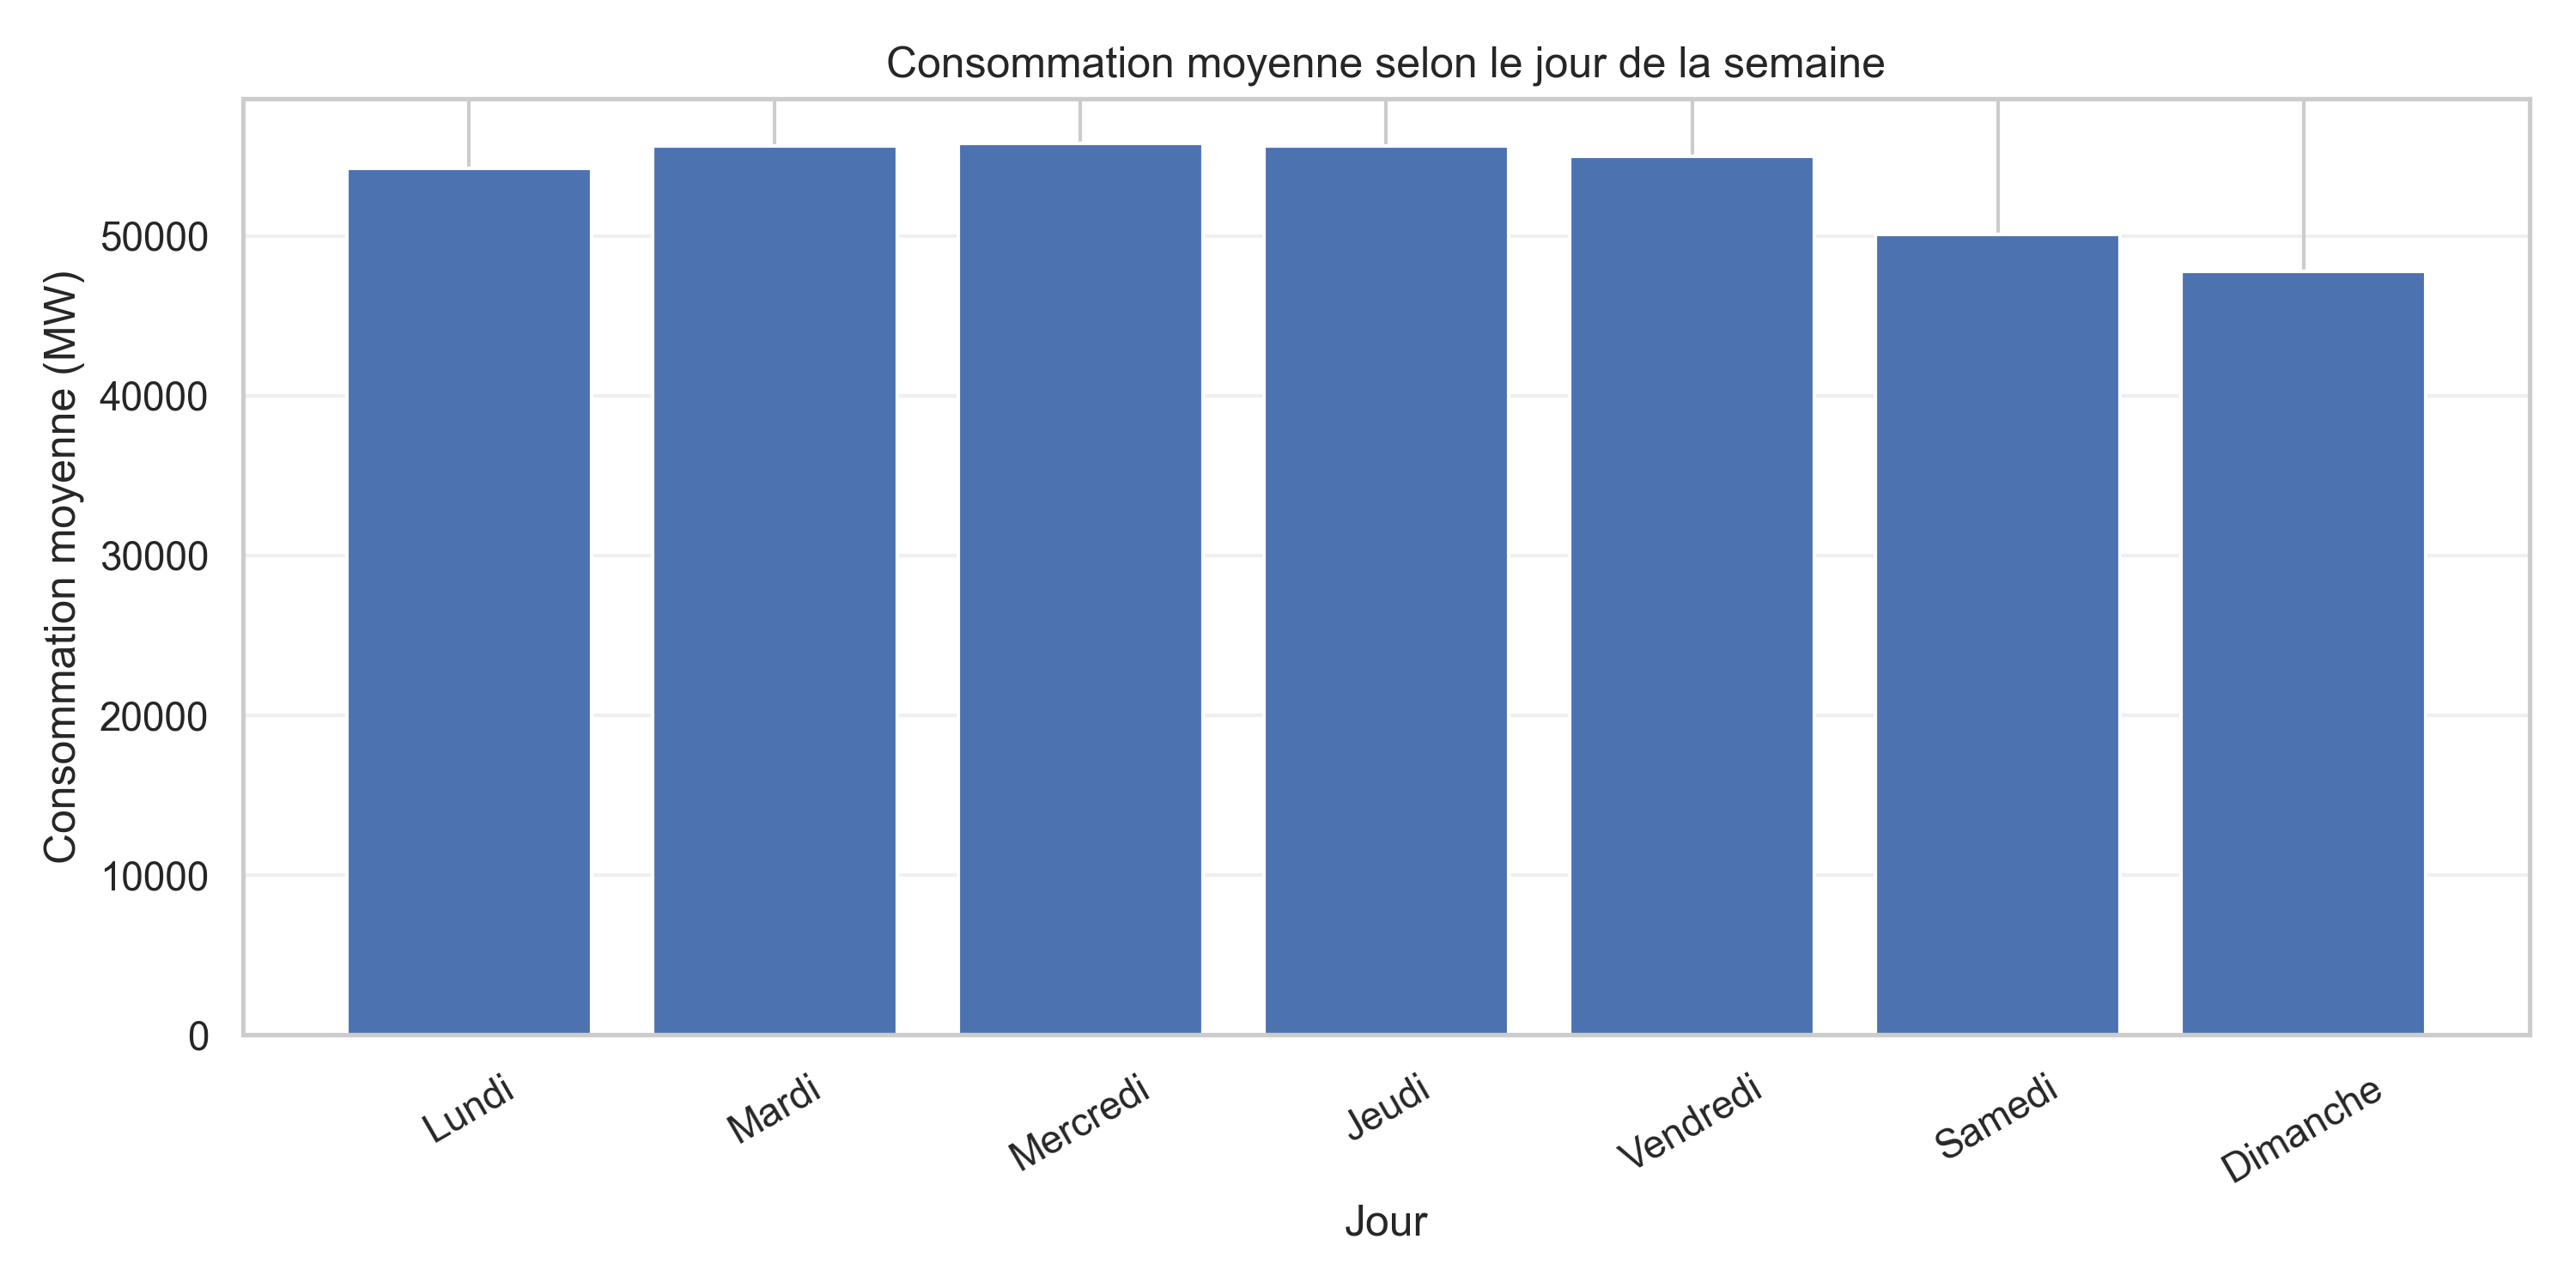
\includegraphics[width=\linewidth]{../results/analyse_2024/exploration/cycle_hebdomadaire.png}\caption{Cycle hebdomadaire.}\end{subfigure}
  \caption{Consommation moyenne selon l'heure et le jour, 2012--2023.}\label{fig:profils}
\end{figure}

\subsection{Validation 2024 et choix du modèle}
Les dix méthodes sont comparées sur les mêmes 338 journées admissibles de 2024, soit 8\,112 heures ; 28 journées ne satisfont pas les critères de disponibilité, notamment autour des changements d'heure. Le tableau~\ref{tab:scores} donne les erreurs horaires, en MW, avec $e_t=C_t-\widehat C_t$.
\begin{table}[htbp]
  \centering\fontsize{9}{11}\selectfont\renewcommand{\arraystretch}{1.08}
  \caption{Scores horaires de validation 2024 sur les 8\,112 mêmes heures (MW).}\label{tab:scores}
  \begin{tabular}{lrrr}\toprule
  Méthode & MAE & RMSE & Biais\\\midrule
  Forêt aléatoire & 1\,644 & 2\,383 & $-146$\\
  Régression linéaire & 2\,015 & 2\,686 & $-390$\\
  Ridge & 2\,041 & 2\,733 & $-297$\\
  Gradient boosting & 2\,324 & 3\,093 & $-647$\\
  ARMA(1,1) & 2\,147 & 3\,291 & $89$\\
  AR(2) & 2\,177 & 3\,298 & $114$\\
  AR(1) & 2\,230 & 3\,408 & $80$\\
  Semaine précédente & 3\,214 & 4\,888 & $257$\\
  Moyenne de quatre semaines & 3\,705 & 5\,413 & $291$\\
  Persistance & 5\,659 & 7\,056 & $-778$\\\bottomrule
  \end{tabular}
\end{table}

La forêt aléatoire a les plus faibles MAE et RMSE : par rapport à la semaine précédente, la RMSE baisse de 51,2\,\%. La régression linéaire est deuxième en RMSE (2\,686~MW). Parmi les modèles statistiques, ARMA(1,1) prédit légèrement mieux qu'AR(2) (3\,291 contre 3\,298~MW), alors que les AIC/BIC d'AR(2) sont plus faibles : AIC de 1\,576\,213 et BIC de 1\,576\,242, contre 1\,578\,311 et 1\,578\,340 pour ARMA(1,1). L'ajustement sur l'apprentissage ne détermine donc pas à lui seul la qualité hors échantillon. La forêt obtient une erreur absolue quotidienne d'énergie de 33\,478~MWh et une erreur absolue sur la valeur de pointe de 1\,818~MW ; la régression linéaire fait légèrement mieux pour ces deux critères (33\,342~MWh et 1\,633~MW).

L'ablation de la forêt aléatoire (figure~\ref{fig:ablation}) donne une RMSE de 6\,031,15~MW avec le seul calendrier, 2\,387,66~MW en ajoutant l'historique de consommation, et 2\,383,19~MW en ajoutant la météo passée. Le gain apporté par cette météo historique est de 4,47~MW (0,19\,\% de la RMSE précédente) ; sa signification statistique n'a pas été évaluée. Il ne permet pas de conclure à l'absence d'un effet physique de la météo.
\begin{figure}[htbp]
  \centering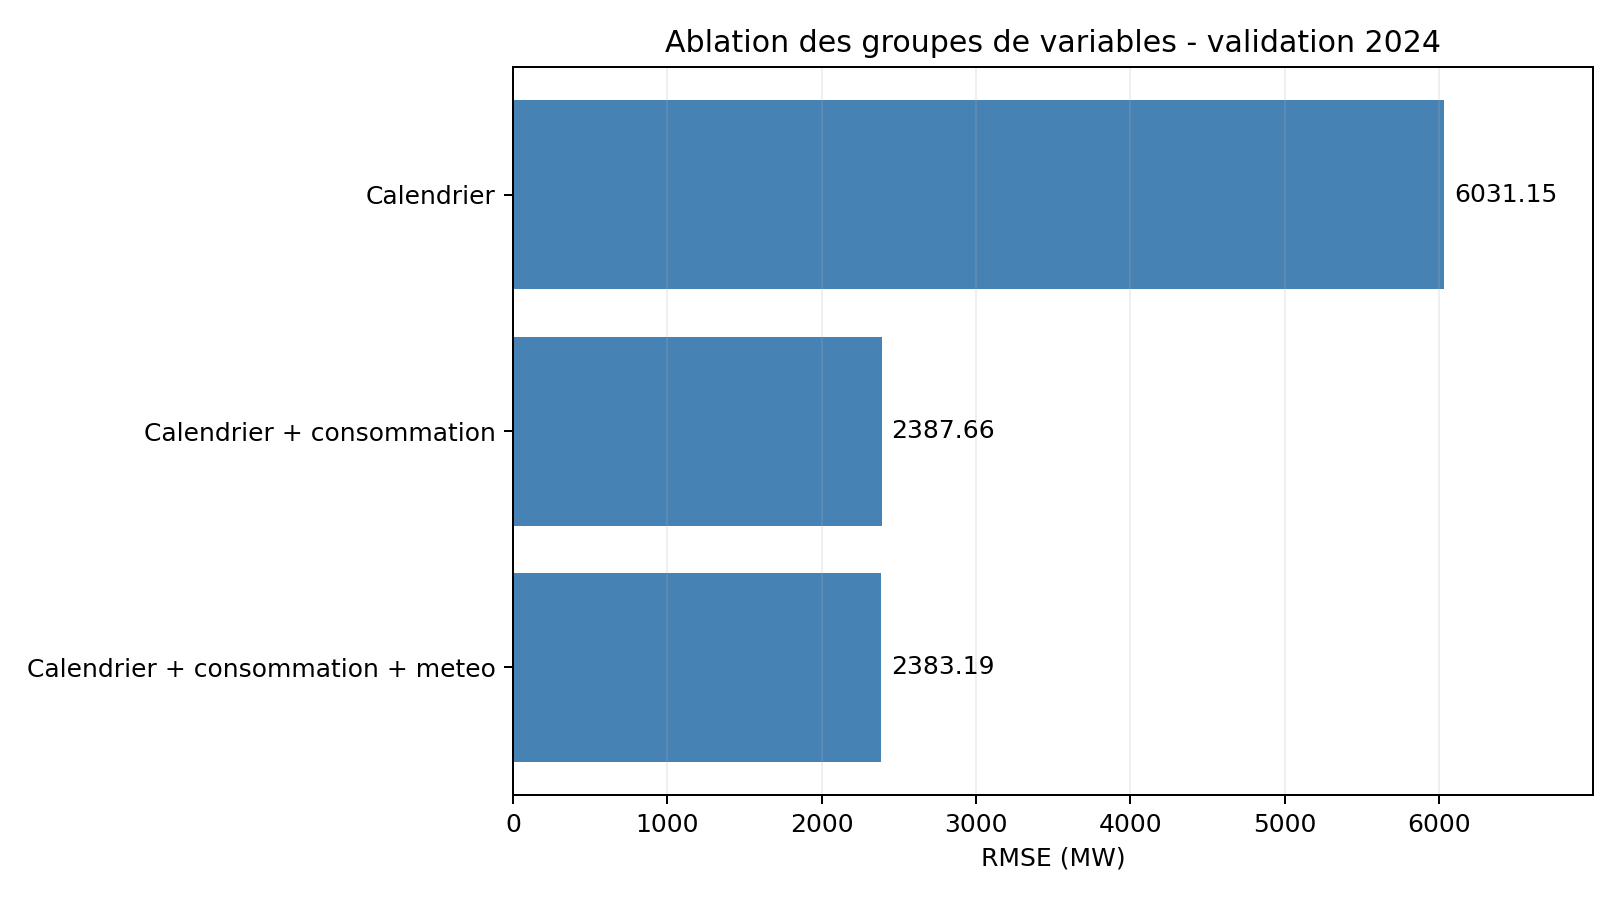
\includegraphics[width=.69\linewidth]{../results/analyse_2024/ablation/comparaison_ablation.png}
  \caption{Ablation des familles de variables en validation 2024 (RMSE).}\label{fig:ablation}
\end{figure}

\subsection{Hétérogénéité et journées difficiles en 2024}
La RMSE de la forêt est de 3\,546~MW en hiver contre 1\,065~MW en été ; elle atteint 3\,175~MW sur les jours fériés et 2\,361~MW sur les autres jours. Seuls huit jours fériés sont évalués. Par température observée, les catégories moins de 5~\textdegree C, 5 à moins de 15~\textdegree C et au moins 15~\textdegree C comptent respectivement 733, 4\,175 et 3\,199 heures ; cinq heures ont une météo manquante. La forêt fait mieux que le benchmark hebdomadaire dans les trois classes renseignées. Ces températures observées ne servent qu'au diagnostic a posteriori, pas à la prévision de $J+1$.

Sur le plus long bloc continu de 4\,320 heures, les ACF des \emph{erreurs de prévision} des AR/ARMA conservent une dépendance ; les tests de Ljung--Box aux retards 24 et 168~h rejettent l'absence d'autocorrélation ($p<0{,}001$). Ces erreurs à plusieurs horizons ne sont pas les innovations à un pas du modèle ajusté.

Les trois journées de plus forte RMSE quotidienne pour la forêt, choisies sur la validation 2024, sont le 24 décembre (surestimation moyenne de 6\,958~MW), le 21 novembre et le 19 janvier (sous-estimations de 7\,118 et 6\,940~MW). La figure~\ref{fig:echecs} illustre ces écarts de niveau malgré des profils horaires globalement suivis. Le 24 décembre n'est pas férié officiellement ; son voisinage de Noël est une explication possible, non démontrée.
\begin{figure}[htbp]
  \centering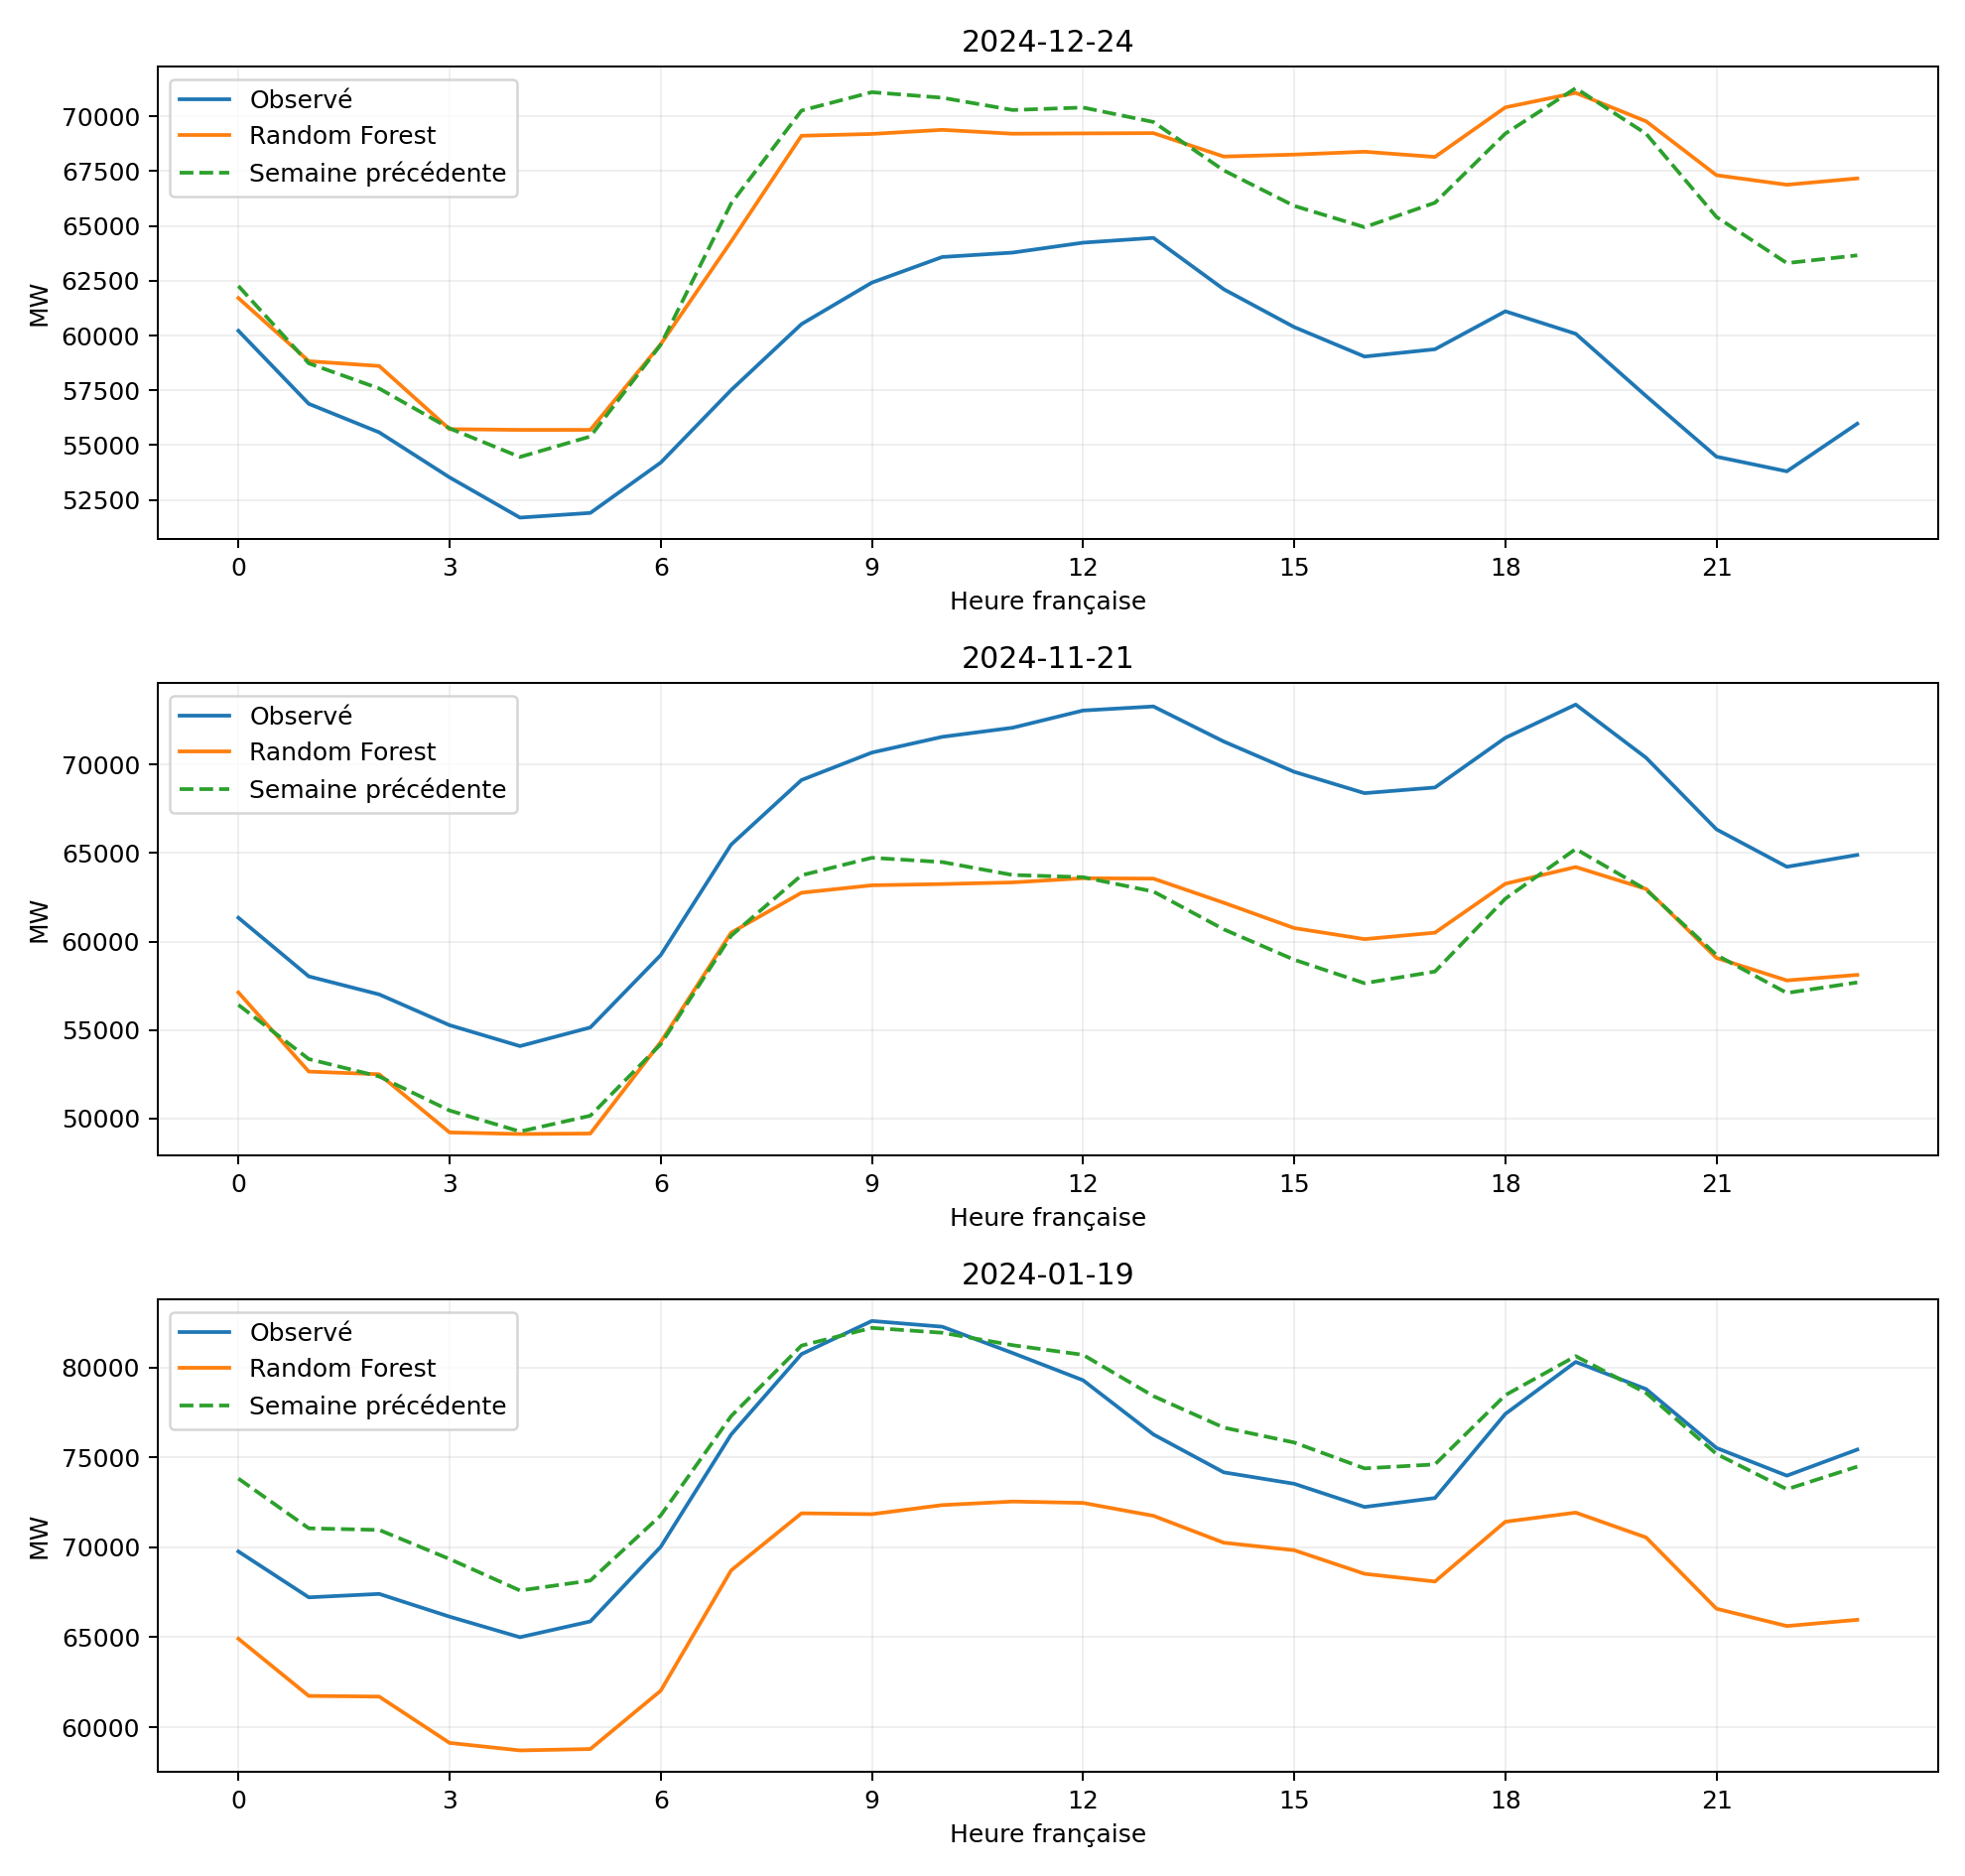
\includegraphics[width=.67\linewidth]{../results/analyse_2024/diagnostics/trois_echecs.png}
  \caption{Trois journées de validation 2024 aux plus fortes RMSE quotidiennes de la forêt aléatoire.}\label{fig:echecs}
\end{figure}

\subsection{Test final indépendant 2025}
Après sélection sur 2024 et réentraînement sur l'historique disponible avant 2025, seule la forêt aléatoire est évaluée en 2025 : 337 journées admissibles, soit 8\,088 heures. Les périodes et effectifs diffèrent entre validation et test ; la comparaison du tableau~\ref{tab:rf_test} décrit la stabilité observée, sans mesurer un gain causal dû au réentraînement.
\begin{table}[htbp]
  \centering\fontsize{9}{11}\selectfont
  \caption{Forêt aléatoire : validation et test final, erreurs horaires en MW.}\label{tab:rf_test}
  \begin{tabular}{lrrrr}\toprule
  Période & Journées & MAE & RMSE & Biais\\\midrule
  Validation 2024 & 338 & 1\,644,14 & 2\,383,19 & $-145,94$\\
  Test 2025 & 337 & 1\,619,14 & 2\,306,95 & $-20,20$\\\bottomrule
  \end{tabular}
\end{table}
\begin{figure}[htbp]
  \centering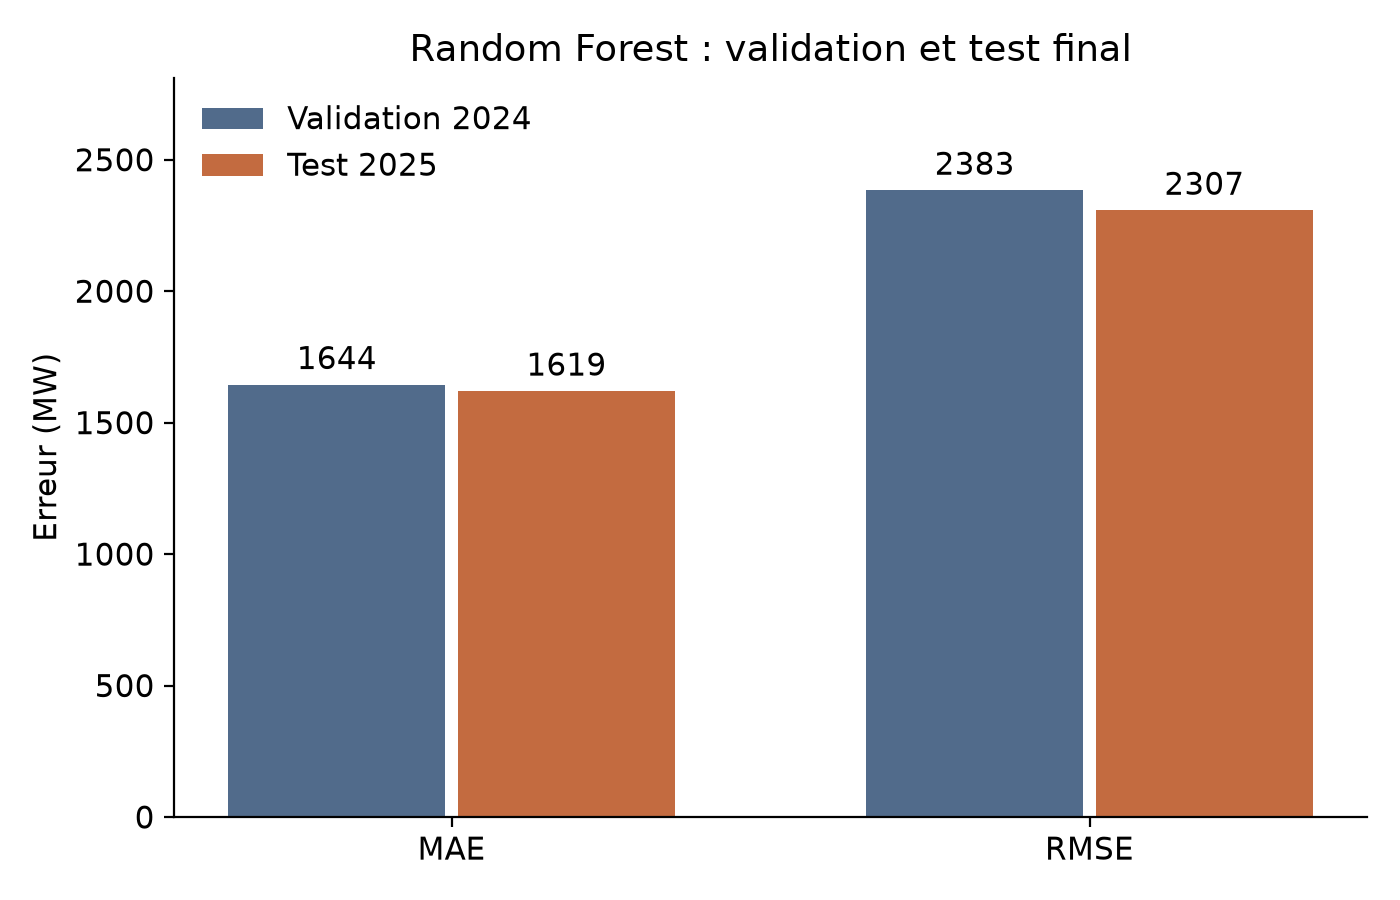
\includegraphics[width=.66\linewidth]{../results/test_2025/figures/comparaison_2024_2025.png}
  \caption{MAE et RMSE de la forêt aléatoire en validation 2024 et en test 2025.}\label{fig:test_comparaison}
\end{figure}

La figure~\ref{fig:test_annee} compare les \emph{moyennes journalières} des observations et des 24 prévisions horaires sur les journées effectivement évaluées en 2025. Les journées exclues ne sont pas interpolées. Pour montrer la forme horaire, la figure~\ref{fig:test_saisons} présente quatre semaines calendaires complètes admissibles, choisies vers le milieu des mois visés sans regarder les erreurs. Aucune semaine complète d'avril ne satisfait ce critère : la semaine du 5 au 11 mai représente donc le printemps. Ces exemples visuels ne suffisent pas à établir des scores saisonniers pour 2025.
\begin{figure}[htbp]
  \centering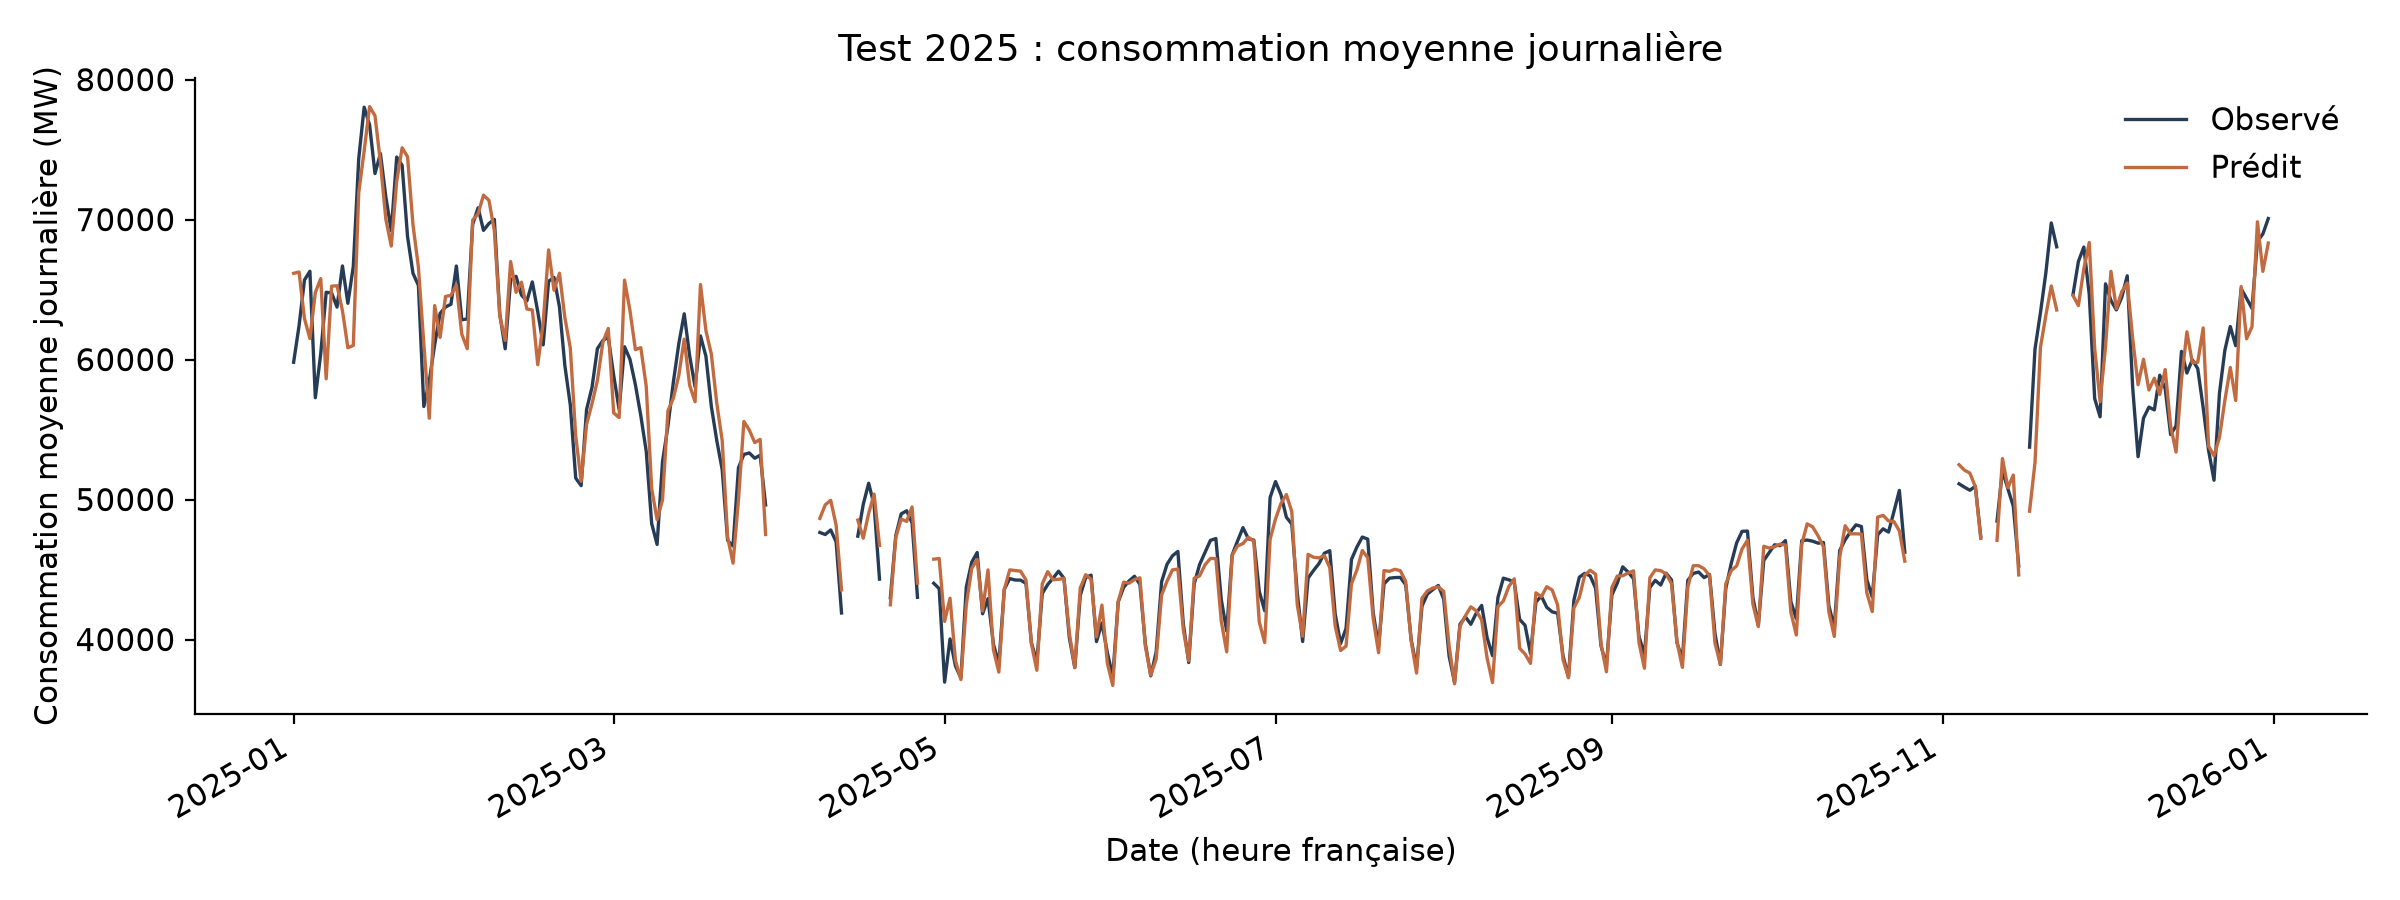
\includegraphics[width=.73\linewidth]{../results/test_2025/figures/observe_vs_predit_annee_2025.png}
  \caption{Consommations moyennes journalières observées et prédites sur les journées admissibles de 2025 (MW).}\label{fig:test_annee}
\end{figure}
\begin{figure}[htbp]
  \centering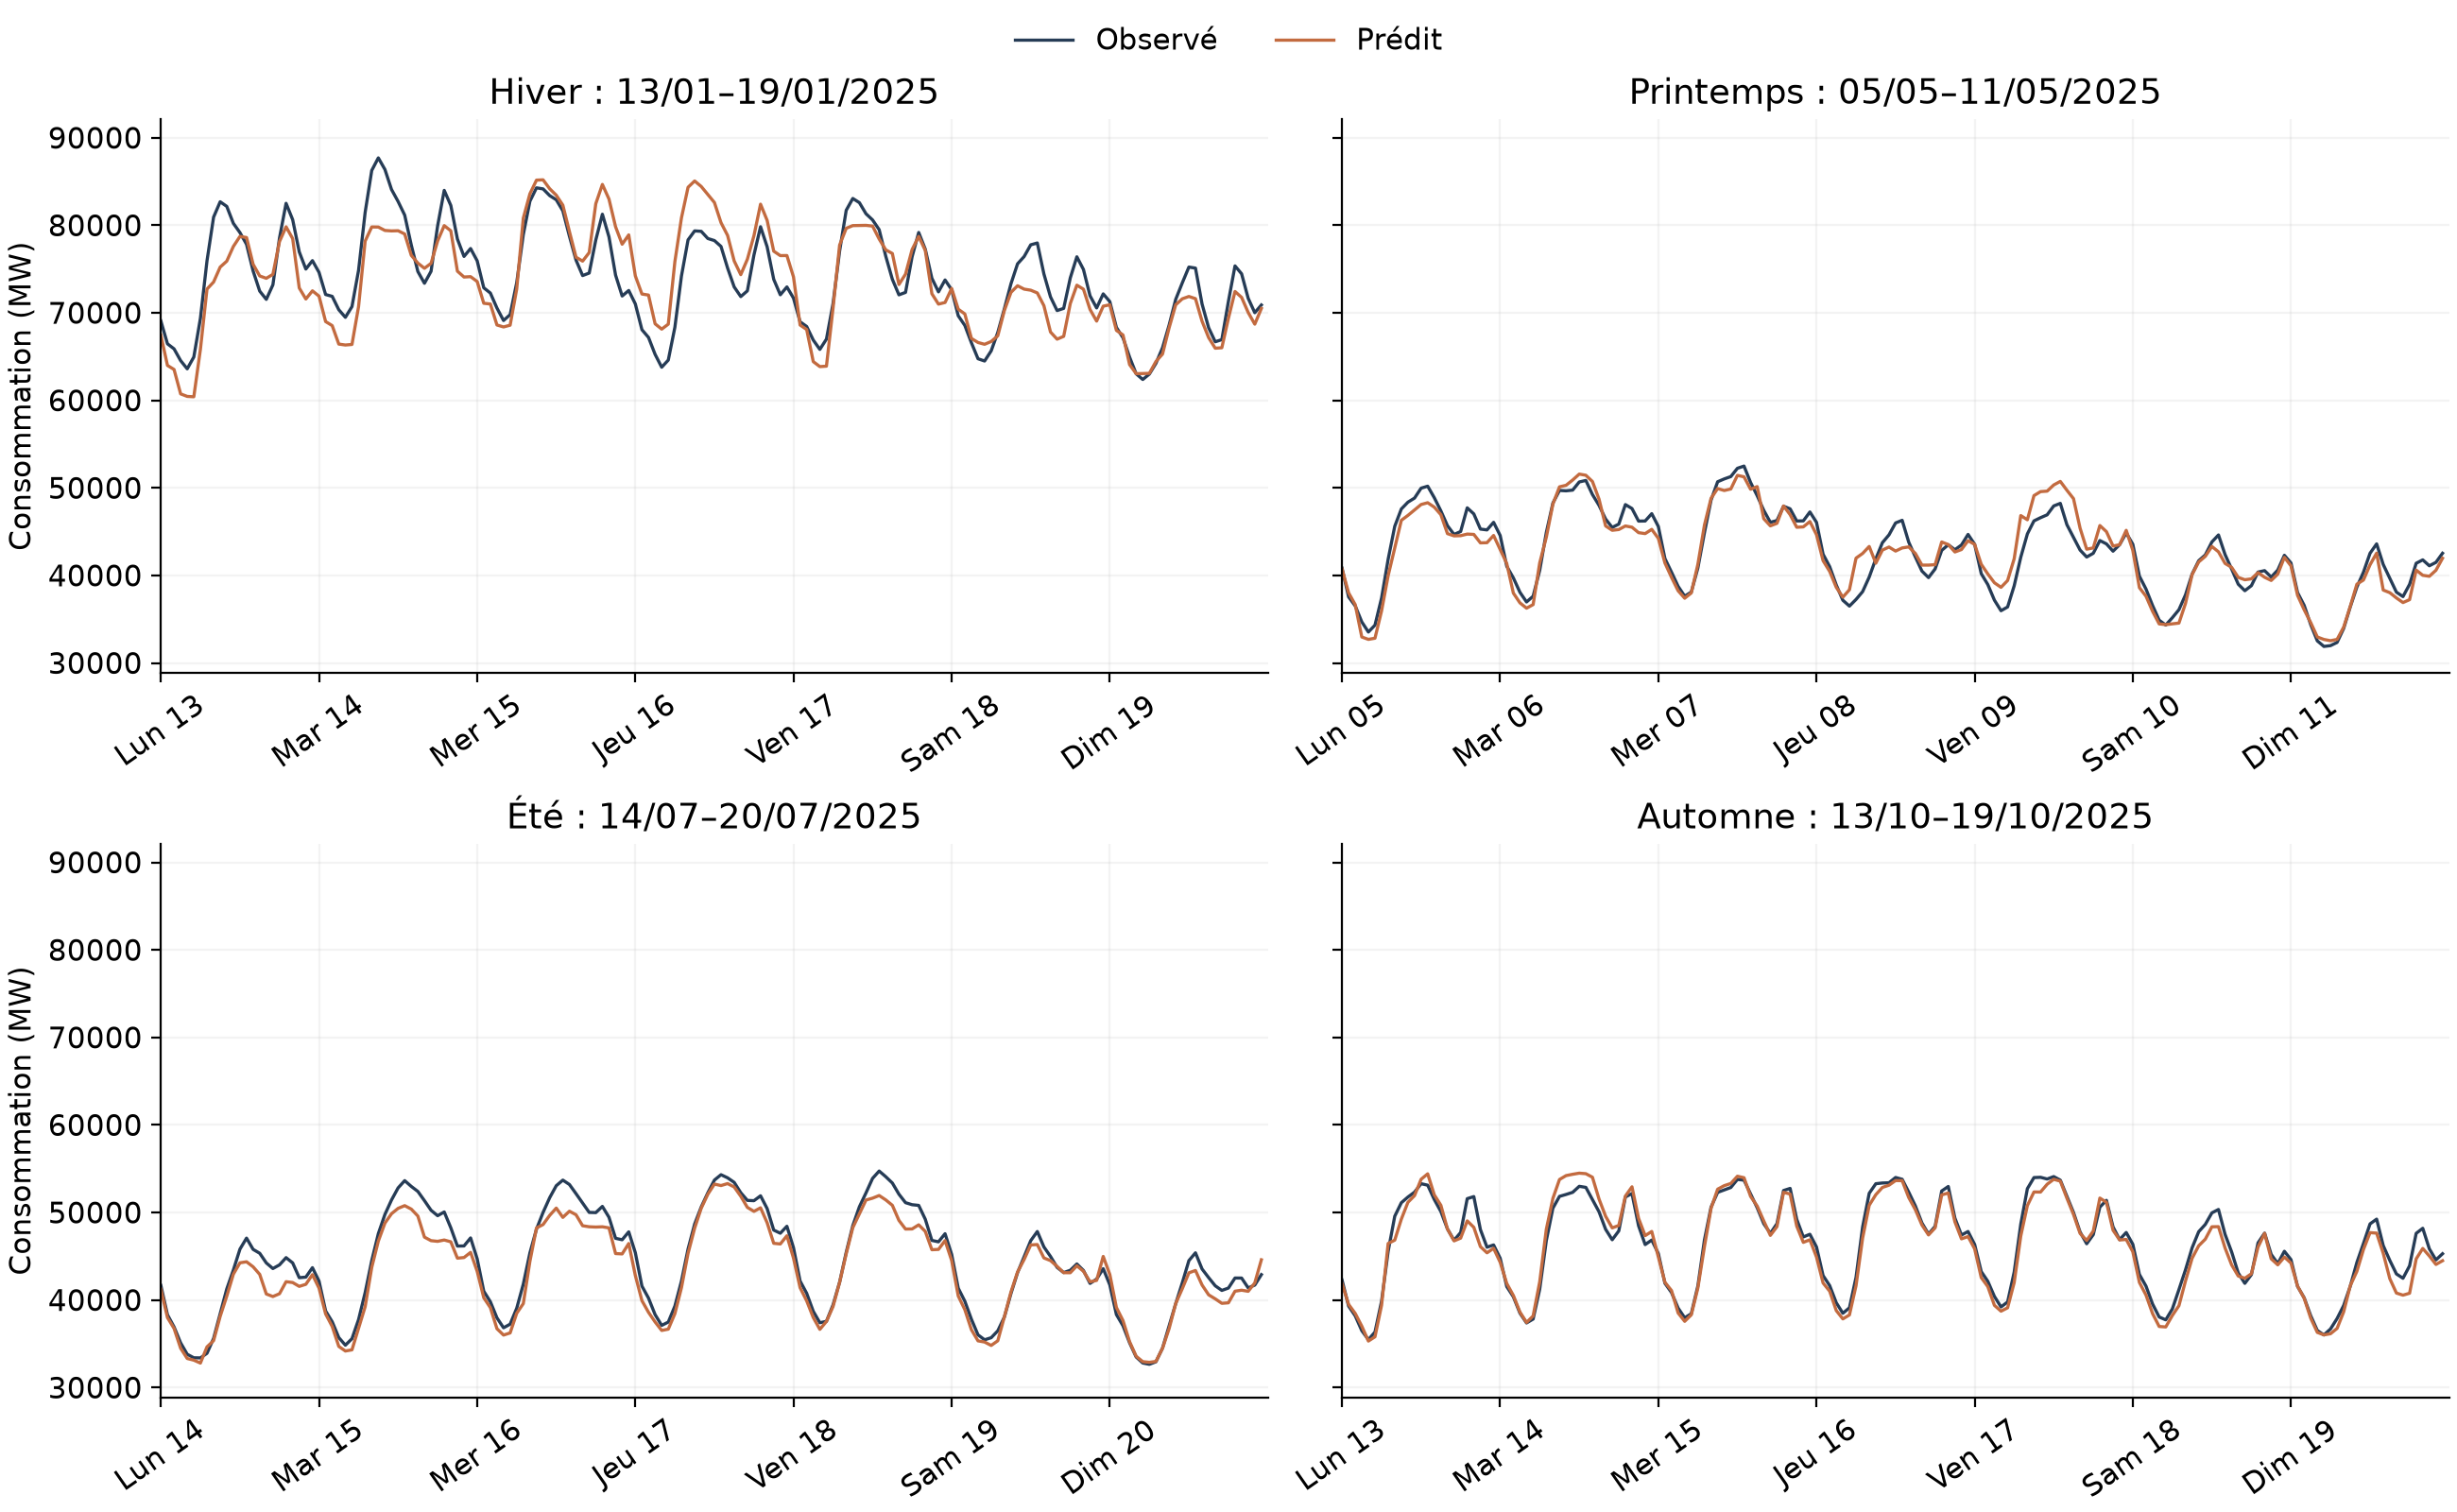
\includegraphics[width=.88\linewidth]{../results/test_2025/figures/observe_vs_predit_2025.png}
  \caption{Valeurs horaires observées et prédites : hiver (13--19 janvier), printemps (5--11 mai), été (14--20 juillet), automne (13--19 octobre 2025). Échelle verticale commune.}\label{fig:test_saisons}
\end{figure}


\section{Discussion}
\noindent

\subsection{Disponibilité des données et risques de fuite}
\noindent

\subsection{Analyse de trois journées d’échec}
\noindent

\subsection{Robustesse et limites des modèles}
\noindent

\subsection{Trois exemples documentés d’usage des agents IA}
\noindent


\newpage

\printbibliography[heading=bibintoc]


\end{document}
